%%%%%%%%%%%%%%%%%%%%%%%%%%%%%%%%%%%%%%%%%%%%%%%%%%%%%%%%%%%%%%%%%%%%%%%%%%%%%%%%%%
%%% Introduction
%%%%%%%%%%%%%%%%%%%%%%%%%%%%%%%%%%%%%%%%%%%%%%%%%%%%%%%%%%%%%%%%%%%%%%%%%%%%%%%%%%
\chapter{Introduction}
	\label{ch::introduction}
	
	\begin{figure}[h!]
		\centering
		\fbox{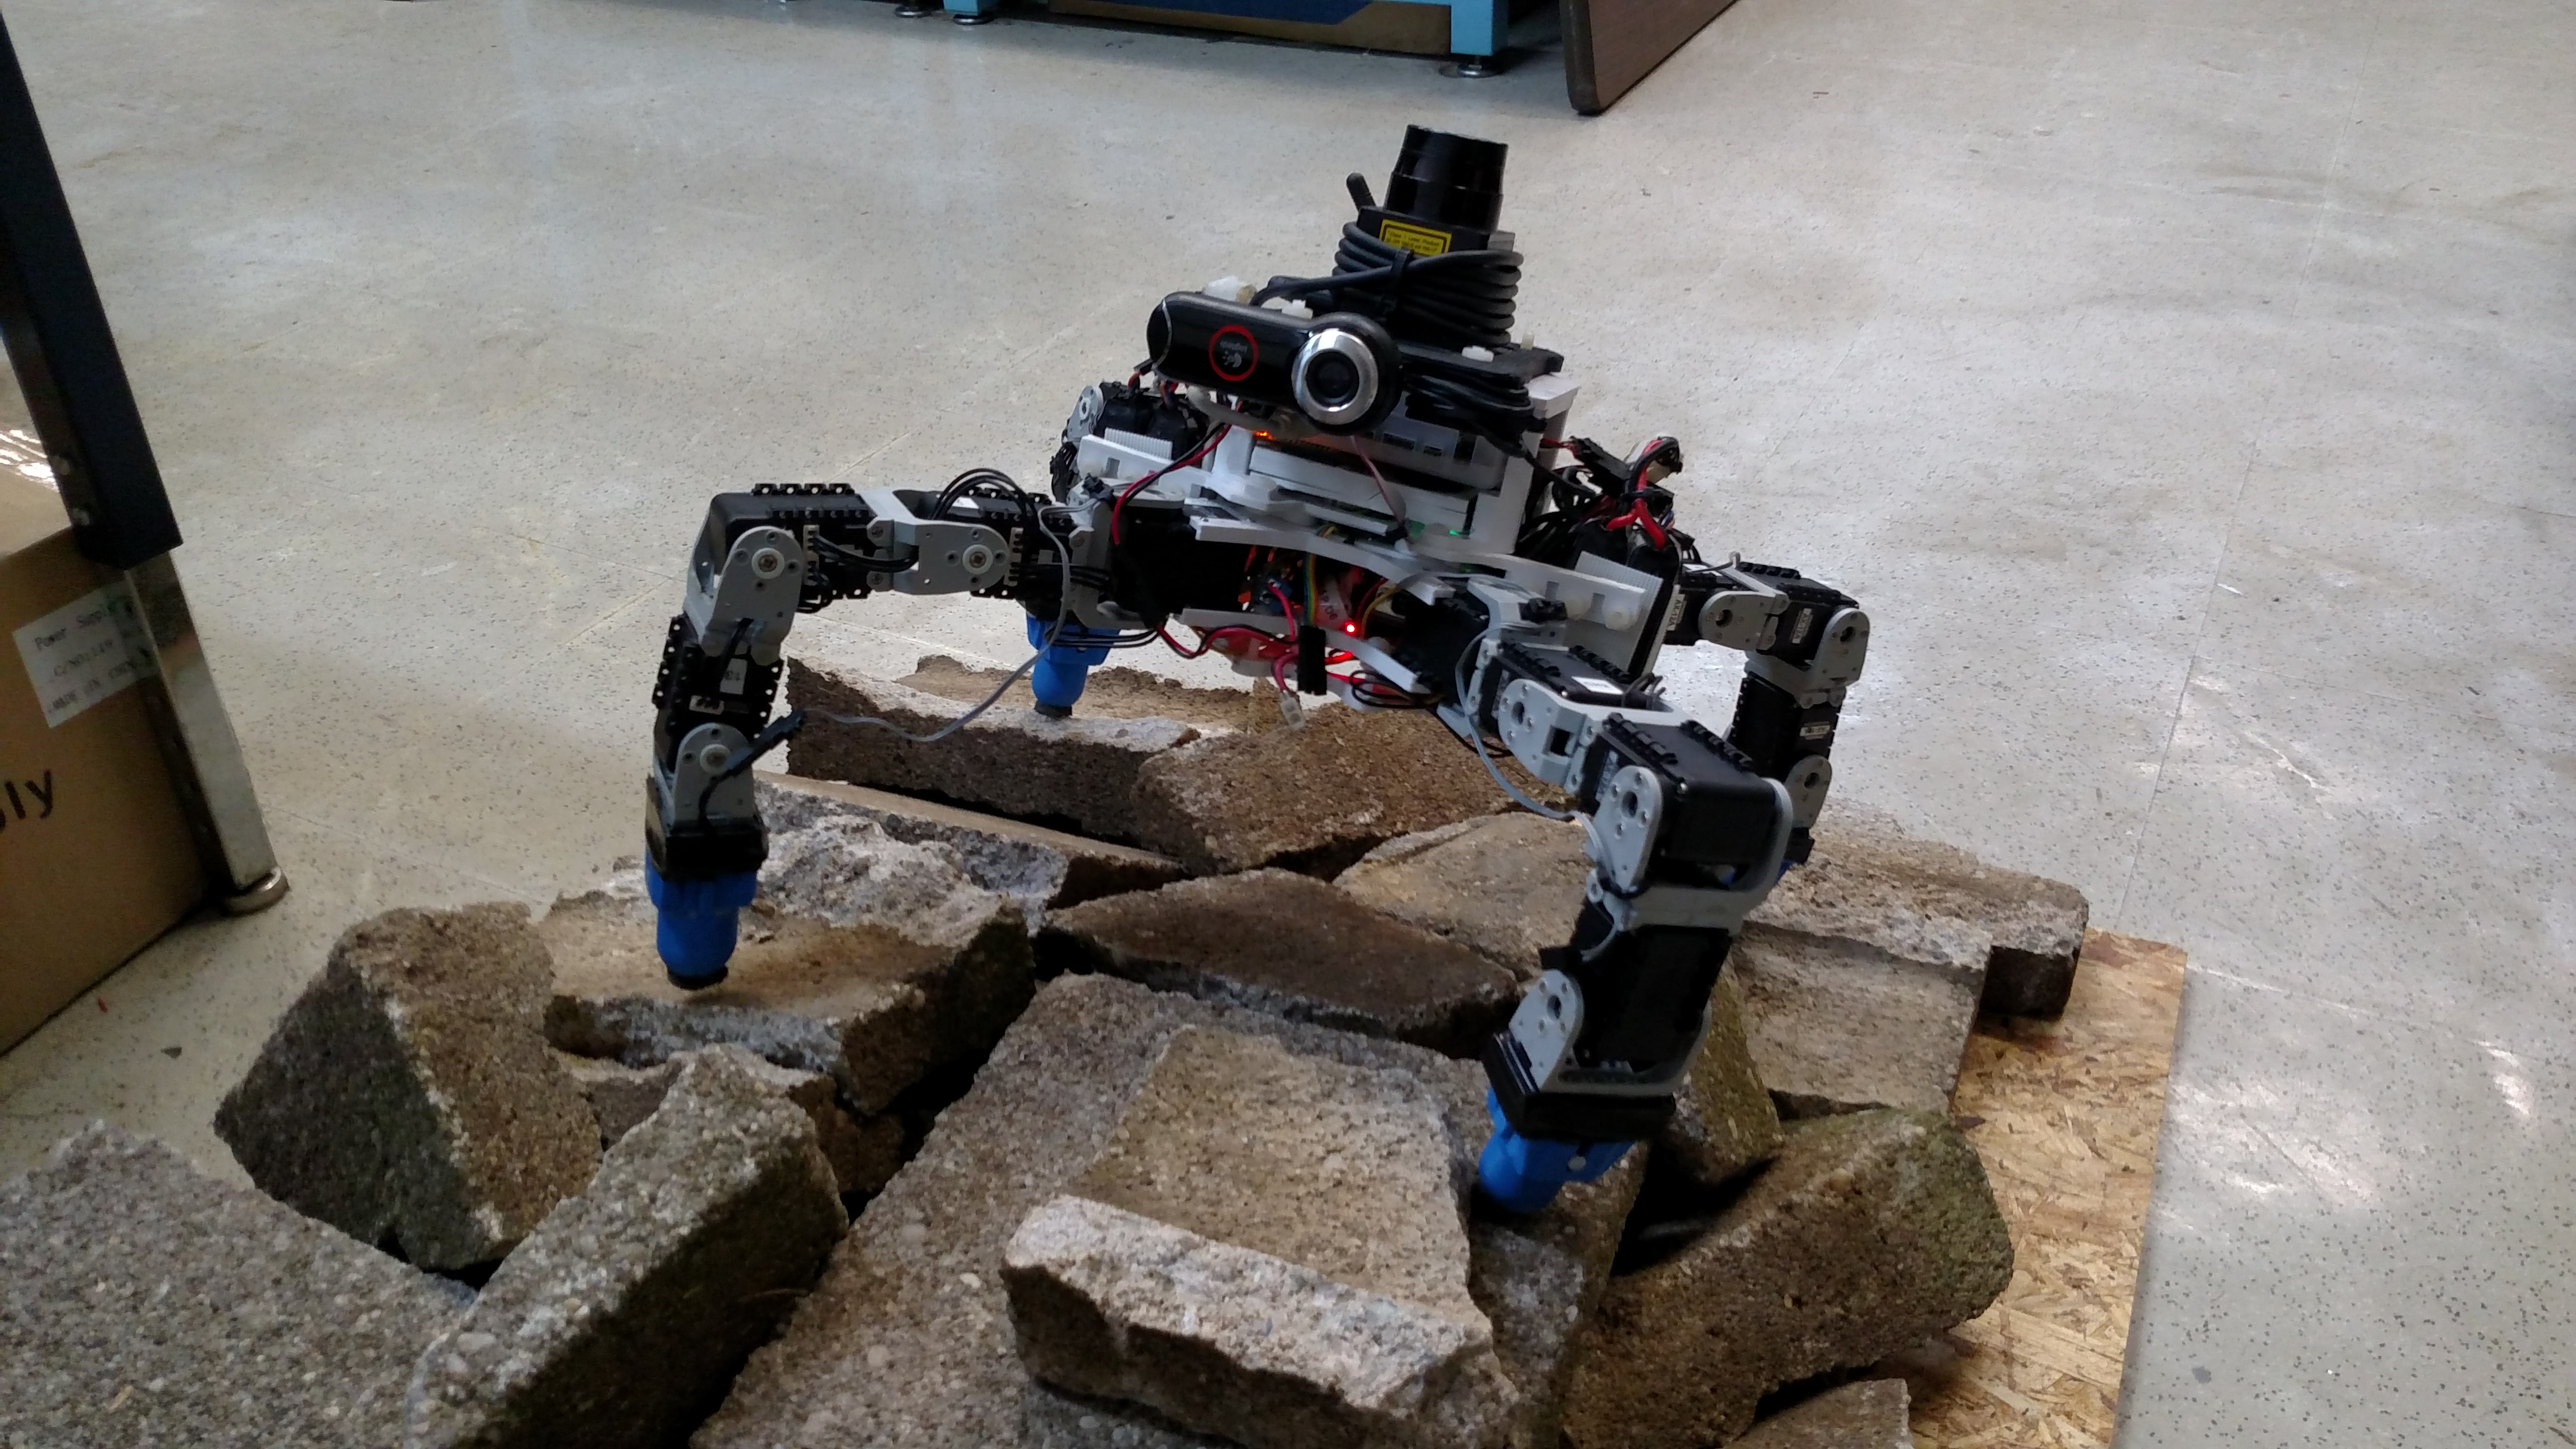
\includegraphics[width=\textwidth]{on_the_rocks2.jpg}}
		\caption{The BlueFoot Quadruped Robot}
		\label{fig::bluefoot_glamour}
	\end{figure}
		The design of legged robots and associated methods of locomotion control has been an area of interest spanning the past several decades, as shown by \cite{McGhee1965,Hodgins1991,Altendorfer2001,Kolter2008,Wieber2015}. Quadruped robotic systems have gained popularity in studies pertaining to variable terrain navigation and full-body stability adaptation. Well known examples of this from the past decade are the Tekken \cite{Fukuoka2003}, Kolt \cite{Estremera2006}, BigDog \cite{BigDog2008}, and HyQ \cite{Semini2010_PHD} quadrupeds. Many of these systems have been implemented on a larger scale so that they can carry substantial payloads while maintaining adequate system bandwidth for fast gaits and robustness to rough terrains. Few, however, have been implemented on the scale of a hobby-robot platform while still maintaining an aptitude for rough terrain navigation and comparable sensory prowess.

		The BlueFoot quadruped is a self-contained, fully-actuated platform with the dexterity to perform stabilization and repositioning maneuvers on variable terrains along the same lines as the LittleDog platform \cite{Rebula2007}. Namely, BlueFoot has been designed with 16 actuated degrees of freedom to allow for the execution of a wide range of body and leg articulation while configured in a large range of kinematic poses. This level of dexterity allows the platform to overcome raised terrain, as well as to independently control the motion of on-board sensors attached to its main trunk. Namely, BlueFoot has the ability to pitch and yaw its on-board camera and LIDAR sensor units without gaiting, simply by reposing its body. BlueFoot also includes a sizable array of other on-board sensors for feedback and control, including joint position, velocity and loading sensors; an inertial measurement unit (IMU); and foot-contact sensors. Using the computational, sensory and motor capacities at hand, BlueFoot has the ability to utilize similar control mechanisms to those implemented on larger quadruped systems, such as those previously referred to. 

		Aside from its design, the BlueFoot platform inherently demands a sizable number of control routines to achieve fluid locomotion and system stability, making this robot an ample platform for studies related to gait design and motion planning. In particular, BlueFoot's controller development has included a large degree of kinematic modeling and open-loop gait design and stabilization for the purpose of achieving dynamic locomotion control. In particular, BlueFoot is gaited via a central pattern generator (CPG) based gaiting algorithm augmented with a foothold controller along the same lines as \cite{Ajallooeian2013} and \cite{Rutishauser2008}. Additionally, active platform stabilization is performed via a zero-moment point (ZMP) based body-posture controller which actively stabilizes the system during arbitrary gaiting sequences. The controllers presented in this thesis make use of virtual-forces to drive system reference commands. An outer-loop controller supplies commands and corrections used in system navigation control.

		

		This report will detail the specific implementations of each of the aforementioned control techniques